\section{Sampling methods and individual curves}\label{app:samplers}
Within each ATLAS architecture and training run, all seven samplers share the same checkpoint. They change how the walks or particles are constructed numerically, not the learned next-state probabilities. The true-generator IID sampler substitutes the known SFSA law for the learned law and serves as a finite-sampling control. Supplementary Section S5 gives the constructions in detail, including the importance weights and the particle updates.

\begin{center}\begin{minipage}{\textwidth}\centering\small
\begin{tabular}{p{0.21\textwidth}p{0.69\textwidth}}\toprule
Method & Construction\\\midrule
IID & Independent uniforms mapped through each walk's next-state categorical distribution.\\
Stratified & Divide $[0,1]$ into $M$ strata, sample once per stratum, and randomly assign the samples to walks at each step.\\
Scrambled Sobol & Assign one randomized low-discrepancy point to each walk; its coordinates supply the successive categorical draws.\\
Antithetic & Pair a uniform vector $U$ with $1-U$, using each path's own conditional probabilities.\\
Importance & Multiply proposed death probabilities by two before normalizing, then correct event and risk counts with likelihood-ratio weights.\\
Weighted branching & Integrate death and dropout exits, expand live successors, and resample $M$ live histories by their probability masses.\\
Conditional MC & Integrate death and dropout exits and sample a conditional live successor for each particle, retaining evolving weights.\\\bottomrule
\end{tabular}
\captionof{table}{The seven numerical methods compared in both experiments. The final two rows use live particles rather than complete observed walks. Branching has three live successors in the single-covariate experiment and seven in the competing-risks experiment.}
\end{minipage}\end{center}

Figure~\ref{fig:individual} shows how individual predicted curves differ across models for three baseline patients.

\begin{center}\begin{minipage}{\textwidth}\centering
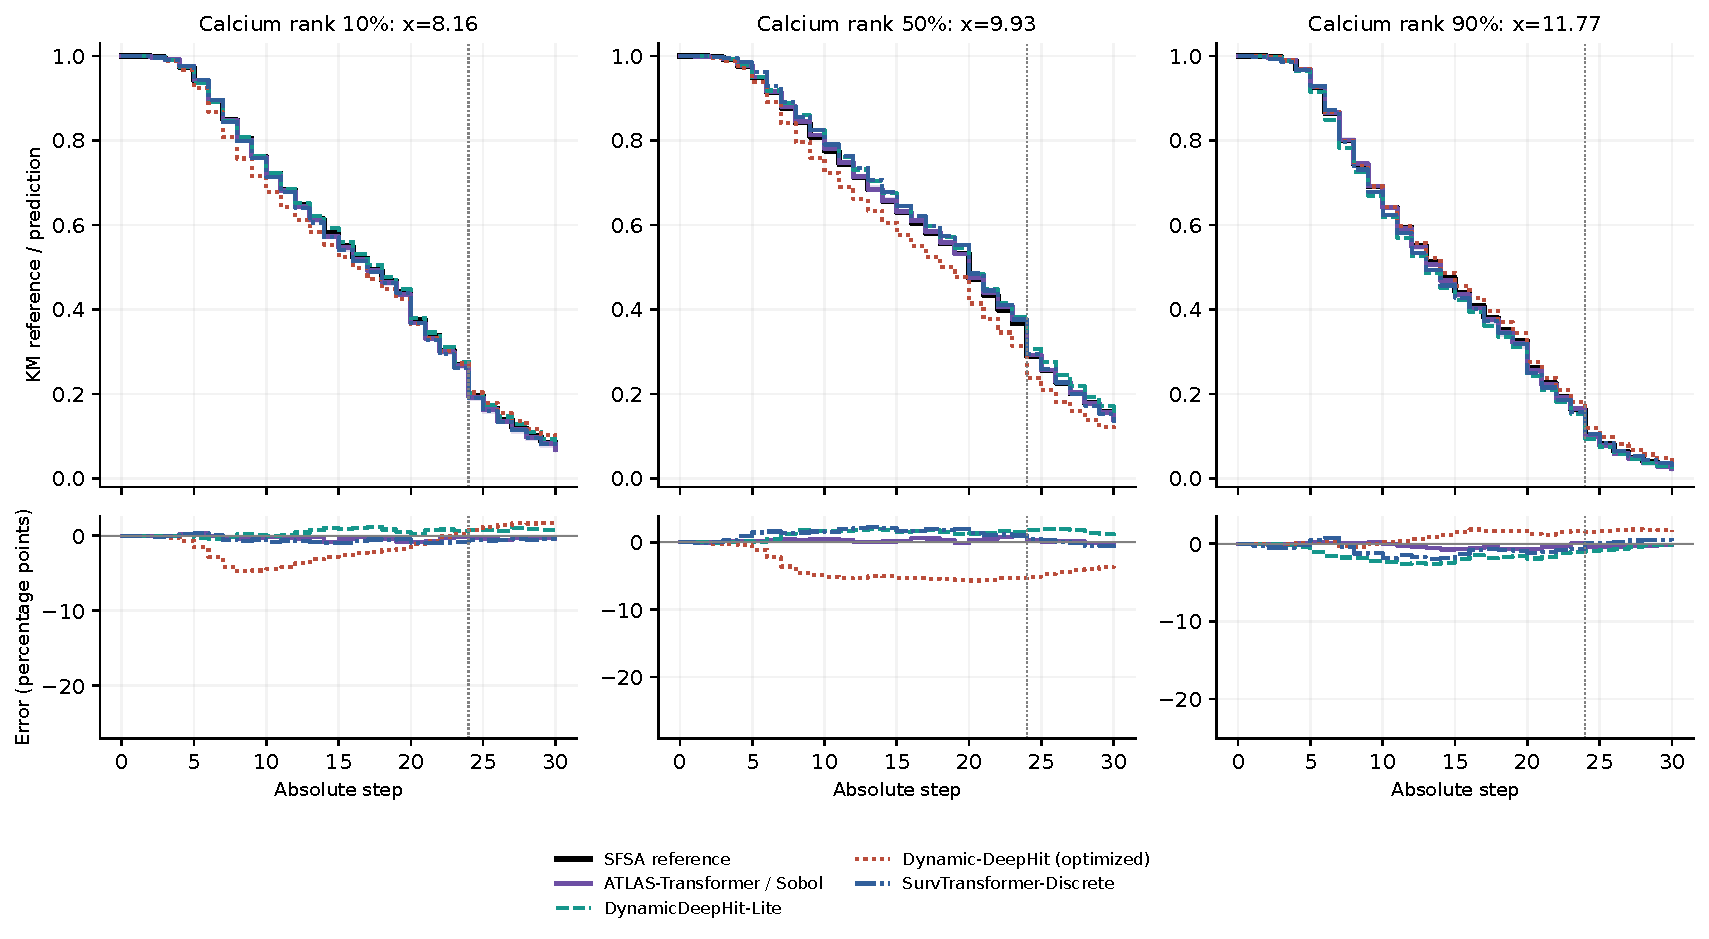
\includegraphics[width=\textwidth]{updated_individual_baseline.pdf}
\captionof{figure}{Individual baseline predictions in the single-covariate duration-dependent experiment. Fitted-model curves use training seed 42; Dynamic-DeepHit (optimized) uses its validation-selected checkpoint. Patients are selected nearest the 10th, 50th and 90th covariate ranks within the 300 scored patients, not by model error. Black is the deterministic reference, and purple is ATLAS-Transformer with Sobol with $M=10{,}000$ and sampling seed 41001. Purple shading is the range across five sampling seeds, not a confidence interval. The other direct-model curves retain their original saved predictions. Lower panels show signed errors in percentage points, and the vertical line marks step 24.}\label{fig:individual}
\end{minipage}\end{center}

Every upper-panel curve is a prediction for one specified covariate value. At baseline there is no observed state prefix. The ATLAS curve comes from 10,000 separately generated futures for that patient, not from walks leading up to the first state and not from pooled walks across different patients. The lower panels show where each curve differs from the reference. A cohort mean prediction curve, by contrast, averages across patients, so overprediction for some and underprediction for others can cancel. The primary MAE in the paper averages individual absolute errors before averaging patients and therefore retains those discrepancies.
